\chapter{Concetti fondamentali del ML}\label{ch-03}

Le lezioni 2 e 3 forniscono la \textbf{panoramica e la terminologia} del
Machine Learning prima di entrare nei modelli veri e propri. Si parte
dal quadro generale --- l'apprendimento come approssimazione di una
funzione sconosciuta a partire da esempi --- per poi descrivere gli
``ingredienti'' di un sistema di ML (dati, task, modello, algoritmo di
apprendimento, validazione) e tre concetti cruciali: il \textbf{bias
induttivo}, la \textbf{funzione di loss} e la \textbf{generalizzazione}.
Molti concetti qui solo accennati verranno ripresi e approfonditi nel
resto del corso.

\section{Il Machine Learning in ambito
computazionale}\label{il-machine-learning-in-ambito-computazionale}

Restringendoci al quadro computazionale, il ML studia \textbf{principi,
metodi e algoritmi per l'apprendimento e la predizione}: il sistema
apprende dall'esperienza (dati noti) per affrontare un compito
computazionale, costruendo un \textbf{modello} (o \textbf{ipotesi}) da
usare per fare predizioni.

Il quadro specifico più diffuso, e quello adottato dal corso, è il
seguente: \textbf{inferire un modello, cioè una funzione, a partire da
un insieme di esempi, in modo che sia capace di generalizzare}, ovvero
di dare risposte accurate su dati nuovi.

\subsection{Quando usare il ML}\label{quando-usare-il-ml}

Il ML va usato con \textbf{opportunità} (quando serve davvero) e
\textbf{consapevolezza} (dei suoi requisiti e limiti). I modelli
predittivi sono utili quando:

\begin{itemize}
\tightlist
\item
  non c'è una teoria (o c'è poca conoscenza) che spieghi il fenomeno;
\item
  i dati sono \textbf{incerti, rumorosi o incompleti}, e questo ostacola
  la formalizzazione di una soluzione esatta.
\end{itemize}

In cambio, il ML richiede due cose: una \textbf{fonte di esperienza} per
l'addestramento (dati \emph{rappresentativi}) e una certa
\textbf{tolleranza sulla precisione} dei risultati, che non saranno mai
garantiti esatti.

Il ML è complementare alle tecniche tradizionali (modelli analitici
basati su conoscenza pregressa, algoritmi e programmazione imperativa,
AI classica). È particolarmente adatto quando:

\begin{itemize}
\tightlist
\item
  \textbf{la conoscenza è troppo difficile da formalizzare} a mano: gli
  esseri umani riconoscono i volti ma non sanno descrivere \emph{come}
  lo fanno; lo stesso vale per il riconoscimento vocale;
\item
  \textbf{la conoscenza umana non basta}: ad esempio prevedere la forza
  di legame di molecole con proteine;
\item
  serve un \textbf{comportamento personalizzato}: filtrare email o
  pagine web secondo le preferenze dell'utente, interfacce uomo-macchina
  individualizzate.
\end{itemize}

Le grandi sfide del ML sono costruire \textbf{sistemi autonomi
intelligenti} (robotica, interazione uomo-robot, motori di ricerca),
fornire \textbf{strumenti potenti per l'analisi dei dati} (gli strumenti
del \emph{data scientist}) e aprire \textbf{nuove aree applicative}
interdisciplinari, in un'epoca in cui il progresso scientifico è sempre
più \emph{data-driven}.

\section{L'apprendimento come approssimazione di
funzioni}\label{lapprendimento-come-approssimazione-di-funzioni}

Il corso adotta una visione specifica ma molto diffusa:
\textbf{l'apprendimento è l'approssimazione di una funzione sconosciuta
a partire da esempi}. Il vantaggio è che task diversi (classificazione,
regressione, \ldots) vengono trattati in un quadro uniforme ---
matematicamente, quello degli spazi di funzioni (spazi di Hilbert) ---
che permette una formulazione rigorosa.

\subsection{L'esempio guida: riconoscimento di
cifre}\label{lesempio-guida-riconoscimento-di-cifre}

Riprendiamo l'esempio della prima lezione. L'input è una collezione di
immagini di cifre scritte a mano (matrici \(8\times 8\) di valori); il
problema è costruire un modello che, ricevuta un'immagine,
\textbf{predica} la cifra. Si tratta di un \textbf{problema di
classificazione} con dieci classi.

È un caso tipico di successo del ML: è \textbf{difficile formalizzare
esattamente} la soluzione (le calligrafie variano, ci sono rumore e dati
ambigui), mentre è \textbf{relativamente facile raccogliere esempi
etichettati}.

\begin{boxdefinition}{Machine Learning (definizione estesa)}

Il ML studia e propone metodi per costruire (\textbf{inferire})
dipendenze, funzioni o ipotesi a partire da esempi di dati osservati,
che: - si \textbf{adattino} agli esempi noti (\emph{fit}); - siano in
grado di \textbf{generalizzare}, con accuratezza ragionevole, su dati
nuovi;

secondo risultati \textbf{verificabili}, sotto condizioni e criteri
statistici e computazionali, tenendo conto dell'\textbf{espressività} e
della \textbf{complessità algoritmica} dei modelli e degli algoritmi di
apprendimento.

\end{boxdefinition}

\subsection{\texorpdfstring{Esempi di coppie
\(x \to f(x)\)}{Esempi di coppie x \textbackslash to f(x)}}\label{esempi-di-coppie-x-to-fx}

In tutti i casi seguenti si vuole inferire una funzione generale
partendo da dati noti, cioè da un \textbf{training set} (TR) di coppie
\(\langle x, f(x)\rangle\):

{\def\LTcaptype{none} % do not increment counter
\begin{longtable}[]{@{}
  >{\raggedright\arraybackslash}p{(\linewidth - 4\tabcolsep) * \real{0.3333}}
  >{\raggedright\arraybackslash}p{(\linewidth - 4\tabcolsep) * \real{0.3333}}
  >{\raggedright\arraybackslash}p{(\linewidth - 4\tabcolsep) * \real{0.3333}}@{}}
\toprule\noalign{}
\begin{minipage}[b]{\linewidth}\raggedright
Problema
\end{minipage} & \begin{minipage}[b]{\linewidth}\raggedright
Input \(x\)
\end{minipage} & \begin{minipage}[b]{\linewidth}\raggedright
Output \(f(x)\)
\end{minipage} \\
\midrule\noalign{}
\endhead
\bottomrule\noalign{}
\endlastfoot
Riconoscimento della scrittura & dati del movimento della penna &
lettera dell'alfabeto \\
Diagnosi medica & proprietà del paziente (sintomi, esami) & malattia o
terapia consigliata \\
Riconoscimento facciale & bitmap del volto & nome della persona \\
Rilevamento spam & messaggio email & spam / non spam \\
\emph{Protein folding} & sequenza di amminoacidi (stringa di lunghezza
variabile) & coordinate 3D degli atomi (sequenza di vettori) \\
\emph{Drug design} & molecola (grafo di atomi e legami) & forza di
legame con la proteasi dell'HIV (numero reale) \\
\end{longtable}
}

Gli ultimi due esempi mostrano che input e output possono essere
\textbf{dati complessi}: stringhe, sequenze, grafi.

\section{Gli ingredienti di un sistema di
ML}\label{gli-ingredienti-di-un-sistema-di-ml}

Un sistema di ML predittivo si può descrivere attraverso i suoi
componenti, che costituiscono anche una \textbf{guida alle scelte
progettuali chiave}.

\begin{figure}[htbp]
\centering
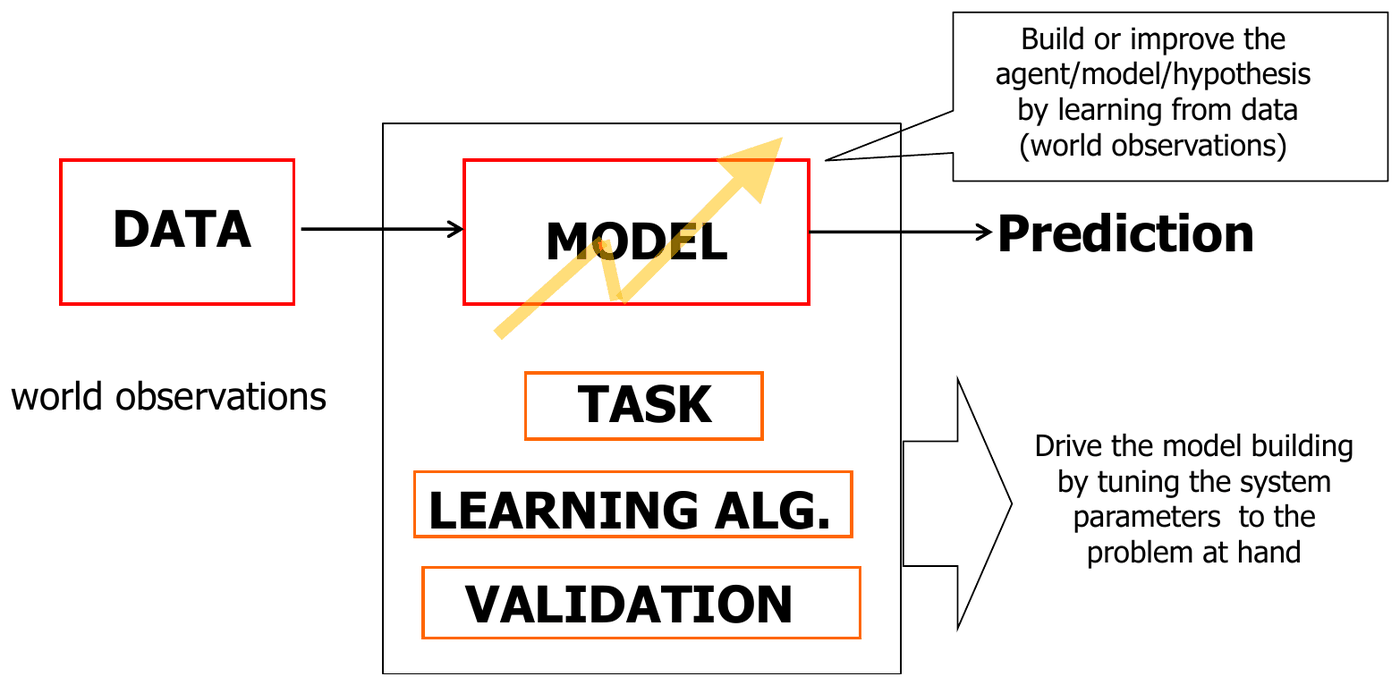
\includegraphics[width=0.86\linewidth,height=0.42\textheight,keepaspectratio]{images/03-l23_sistema-ml.png}
\caption{Panoramica di un sistema di ML predittivo e dei suoi ``ingredienti''.}
\end{figure}

\begin{itemize}
\tightlist
\item
  \textbf{Dati}: le osservazioni del mondo, cioè l'esperienza
  disponibile.
\item
  \textbf{Task}: lo scopo dell'applicazione, che definisce cosa vogliamo
  ottenere.
\item
  \textbf{Modello}: l'agente/ipotesi che viene costruito o migliorato
  apprendendo dai dati.
\item
  \textbf{Algoritmo di apprendimento}: guida la costruzione del modello
  regolando i parametri del sistema sul problema.
\item
  \textbf{Validazione}: valuta la qualità del modello ottenuto.
\end{itemize}

\subsection{Dati}\label{dati}

I dati rappresentano i fatti disponibili. Il primo problema è quello
della \textbf{rappresentazione}: come catturare la struttura degli
oggetti analizzati.

Nel caso \textbf{piatto} (\emph{flat}, linguaggio attributo-valore) ogni
oggetto è un \textbf{vettore di dimensione fissa di proprietà}
(\emph{feature}), e l'intero dataset è una tabella di tuple. Gli
attributi possono essere \textbf{categorici/discreti} (colore: giallo,
rosso) o \textbf{continui} (peso, costo), e possono esserci \textbf{dati
mancanti} (indicati con ``?'').

\begin{boxnote}{Terminologia sui dati}

\begin{itemize}
\tightlist
\item
  Ogni riga \(\mathbf{x}\) (vettore, in grassetto) è un
  \textbf{esempio}, \emph{pattern}, istanza, campione.
\item
  La \textbf{dimensione del dataset} è il numero di esempi, indicato con
  \(l\).
\item
  La \textbf{dimensione dell'input} è il numero di feature, indicato con
  \(n\).
\item
  \(x_i\) (o \(x_j\)) è tipicamente la \(i\)-esima feature (attributo,
  componente) di \(\mathbf{x}\).
\item
  \(\mathbf{x}_p\) è tipicamente il \(p\)-esimo pattern (riga) del
  dataset.
\item
  \(x_{p,i}\) è l'attributo \(i\) del pattern \(p\).
\end{itemize}

\end{boxnote}

I dati possono essere \textbf{pre-elaborati}: scalatura delle variabili,
codifica, selezione delle feature.

\subsubsection{Codifica delle variabili
categoriche}\label{codifica-delle-variabili-categoriche}

Per usare variabili categoriche in modelli numerici bisogna codificarle:

\begin{itemize}
\tightlist
\item
  per \textbf{due classi} si usa \(0/1\) oppure \(-1/+1\);
\item
  per \textbf{più classi} si può usare \(1, 2, 3, \dots\), ma questa
  codifica introduce un \textbf{grado di somiglianza} artificiale (la
  classe 1 risulta ``più vicina'' alla 2 che alla 3). È adatta solo per
  variabili \textbf{categoriche ordinate} (es. piccolo, medio, grande);
\item
  per simboli senza ordine si usa la codifica \textbf{1-of-k} (o
  \textbf{one-hot}): ogni simbolo diventa un vettore con un solo 1, ad
  esempio \(A = (1,0,0)\), \(B = (0,1,0)\), \(C = (0,0,1)\). Tutti i
  simboli sono così equidistanti tra loro. Si usa sia per l'input sia
  per l'output, ed è utile per il progetto.
\end{itemize}

\subsubsection{Dati strutturati}\label{dati-strutturati}

Molti dati non sono naturalmente vettori: \textbf{sequenze} (liste),
\textbf{alberi}, \textbf{grafi}, dati multi-relazionali. Esempi:
immagini, serie temporali, stringhe di un linguaggio, DNA e proteine,
relazioni gerarchiche, molecole, la rete di link delle pagine web. Il
problema è trovare una rappresentazione naturale per essi (se ne parlerà
nella parte avanzata del corso).

\begin{figure}[htbp]
\centering
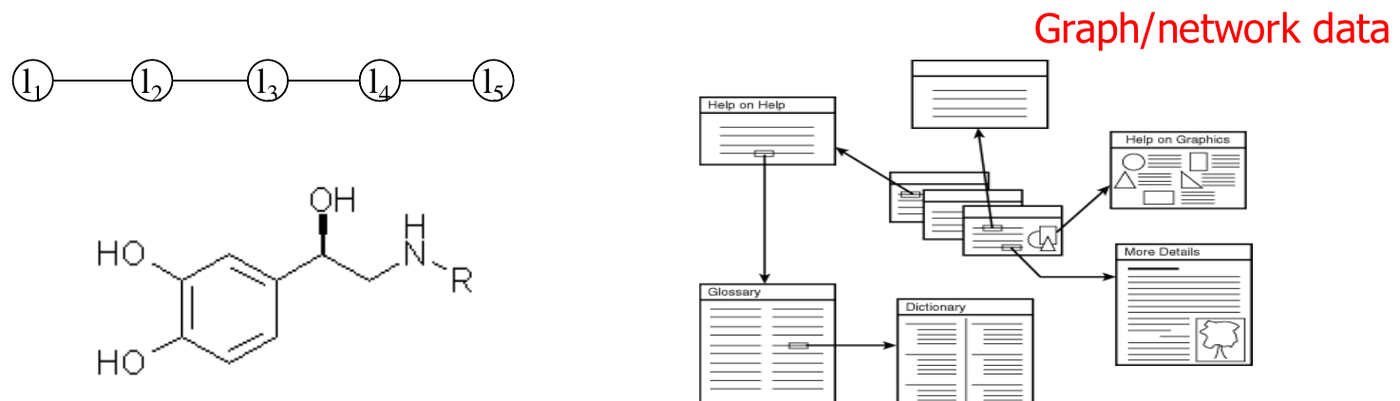
\includegraphics[width=0.74\linewidth,height=0.42\textheight,keepaspectratio]{images/03-l23_dati-strutturati.png}
\caption{Dati strutturati: sequenze, molecole e grafi.}
\end{figure}

\subsubsection{Rumore, outlier e feature
selection}\label{rumore-outlier-e-feature-selection}

\begin{itemize}
\tightlist
\item
  Il \textbf{rumore} (\emph{noise}) è l'aggiunta di fattori esterni al
  segnale informativo: è dovuto alla casualità delle misure, non alla
  legge sottostante (es. rumore gaussiano).
\item
  Gli \textbf{outlier} sono valori insoliti, incoerenti con la maggior
  parte delle osservazioni (es. errori di misura anomali). Si gestiscono
  rilevandoli e rimuovendoli in pre-elaborazione oppure usando metodi di
  modellazione \textbf{robusti}.
\item
  La \textbf{feature selection} seleziona un piccolo numero di feature
  informative, fornendo una rappresentazione ottimale dell'input per il
  problema.
\end{itemize}

\subsection{Task}\label{task}

Il task definisce lo scopo dell'applicazione: quale conoscenza vogliamo
ottenere, qual è la natura utile del risultato, quali informazioni sono
disponibili. Distinguiamo:

\begin{itemize}
\tightlist
\item
  \textbf{task predittivi} (classificazione, regressione):
  approssimazione di funzioni --- sono il focus del corso;
\item
  \textbf{task descrittivi} (cluster analysis, regole di associazione):
  trovare sottoinsiemi o gruppi di dati non classificati.
\end{itemize}

\subsubsection{Apprendimento
supervisionato}\label{apprendimento-supervisionato}

\begin{boxdefinition}{Apprendimento supervisionato}

\textbf{Dati}: esempi di training nella forma
\(\langle \text{input}, \text{output}\rangle = \langle \mathbf{x}, d\rangle\)
(esempi \textbf{etichettati}) per una funzione sconosciuta \(f\), nota
solo nei punti degli esempi. Il \textbf{target} \(d\) (indicato anche
con \(t\) o \(y\)) è fornito da un ``insegnante'' secondo
\(f(\mathbf{x})\).

\textbf{Obiettivo}: trovare una buona approssimazione di \(f\), cioè
un'\textbf{ipotesi} \(h\) utilizzabile per predire su dati mai visti
\(\mathbf{x}'\) --- un'ipotesi che \textbf{generalizzi}.

\end{boxdefinition}

Il target può essere:

\begin{itemize}
\tightlist
\item
  \textbf{categorico} → \textbf{classificazione}:
  \(f(\mathbf{x}) \in \{1, 2, \dots, K\}\) (funzione a valori discreti);
\item
  \textbf{numerico} → \textbf{regressione}:
  \(f(\mathbf{x}) \in \mathbb{R}\) o \(\mathbb{R}^K\) (funzione a valori
  reali continui).
\end{itemize}

Grazie al formalismo dell'approssimazione di funzioni, classificazione e
regressione hanno una \textbf{visione unificata}. In terminologia
statistica gli input sono le \textbf{variabili indipendenti} e gli
output le \textbf{variabili dipendenti} o \textbf{risposte}.

\subsubsection{Apprendimento non
supervisionato}\label{apprendimento-non-supervisionato}

Nell'apprendimento \textbf{non supervisionato} non c'è insegnante: il
training set contiene solo dati \textbf{non etichettati}
\(\langle \mathbf{x}\rangle\). L'obiettivo è ad esempio trovare
\textbf{raggruppamenti naturali} nei dati (\textbf{clustering}, cioè
partizionare i dati in sottoinsiemi di elementi ``simili''), fare
\textbf{riduzione di dimensionalità}, visualizzazione o
pre-elaborazione, oppure \textbf{modellare la densità} dei dati.

\begin{figure}[htbp]
\centering
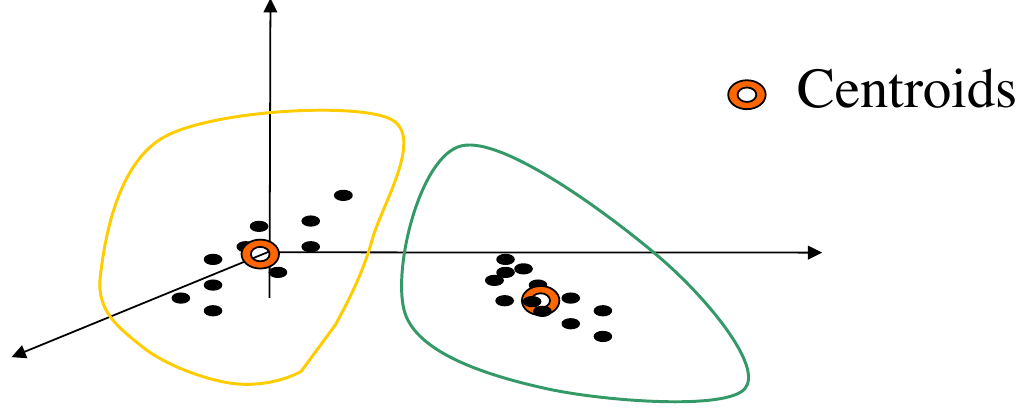
\includegraphics[width=0.60\linewidth,height=0.42\textheight,keepaspectratio]{images/03-l23_clustering.png}
\caption{Clustering: partizione dei dati in gruppi, ognuno rappresentato dal suo
centroide.}
\end{figure}

\subsubsection{Classificazione}\label{classificazione}

Nella classificazione i pattern sono visti come membri di una classe, e
l'obiettivo è assegnare a ogni pattern la classe corretta. Se le classi
sono \textbf{due}, \(f(\mathbf{x})\) è una \textbf{funzione booleana}:
si parla di \textbf{classificazione binaria} o \textbf{concept learning}
(vero/falso, \(0/1\), \(-1/+1\), negativo/positivo). Con \textbf{più di
due} classi si ha un problema \textbf{multi-classe}.

Geometricamente, la classificazione può essere vista come la
\textbf{suddivisione dello spazio degli input in regioni di decisione}.
L'esempio più semplice è il separatore lineare in \(\mathbb{R}^2\): una
retta (in generale un iperpiano) che divide i punti della classe 1 da
quelli della classe 0.

\begin{figure}[htbp]
\centering
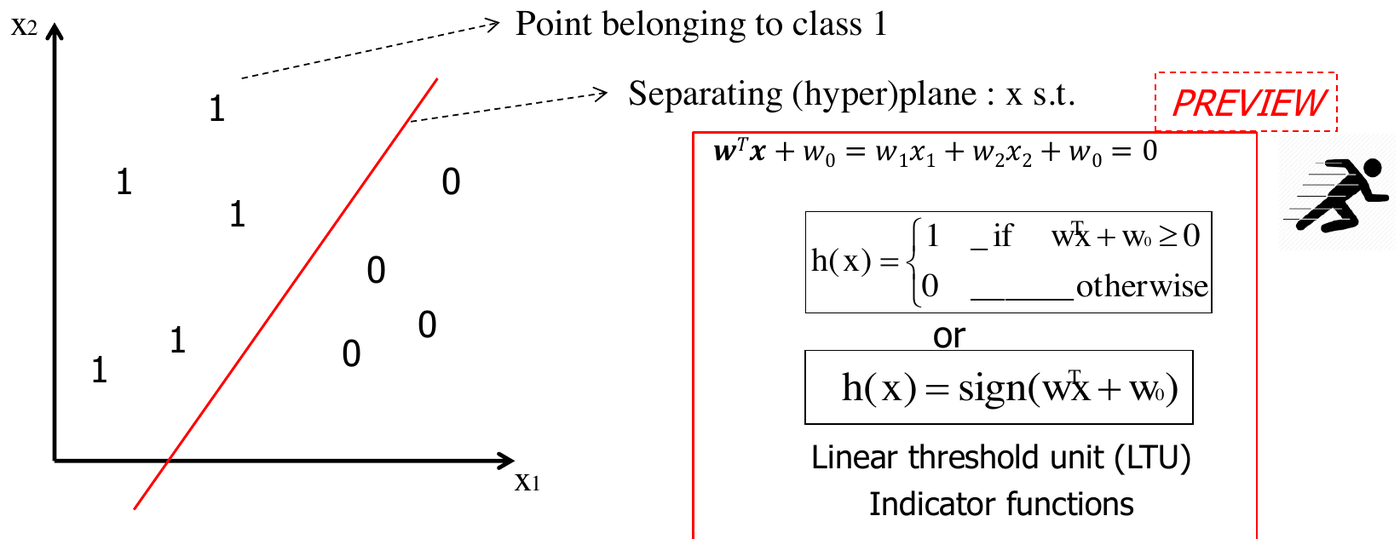
\includegraphics[width=0.89\linewidth,height=0.42\textheight,keepaspectratio]{images/03-l23_separatore-lineare.png}
\caption{Un separatore lineare nel piano: anticipazione della Linear Threshold
Unit.}
\end{figure}

L'iperpiano separatore è l'insieme dei punti \(\mathbf{x}\) tali che \[
\mathbf{w}^T\mathbf{x} + w_0 = w_1 x_1 + w_2 x_2 + w_0 = 0,
\] e il classificatore è \[
h(\mathbf{x}) = \begin{cases} 1 & \text{se } \mathbf{w}^T\mathbf{x} + w_0 \ge 0 \\ 0 & \text{altrimenti} \end{cases}
\qquad \text{oppure} \qquad h(\mathbf{x}) = \operatorname{sign}(\mathbf{w}^T\mathbf{x} + w_0).
\] Questo modello si chiama \textbf{Linear Threshold Unit} (LTU) e sarà
studiato in dettaglio più avanti. Funzioni di questo tipo, a valori in
\(\{0,1\}\), sono dette \textbf{funzioni indicatrici}. L'insieme \(H\)
di tutte le dicotomie (divisioni in due classi) indotte dagli iperpiani
è il suo spazio delle ipotesi.

\begin{figure}[htbp]
\centering
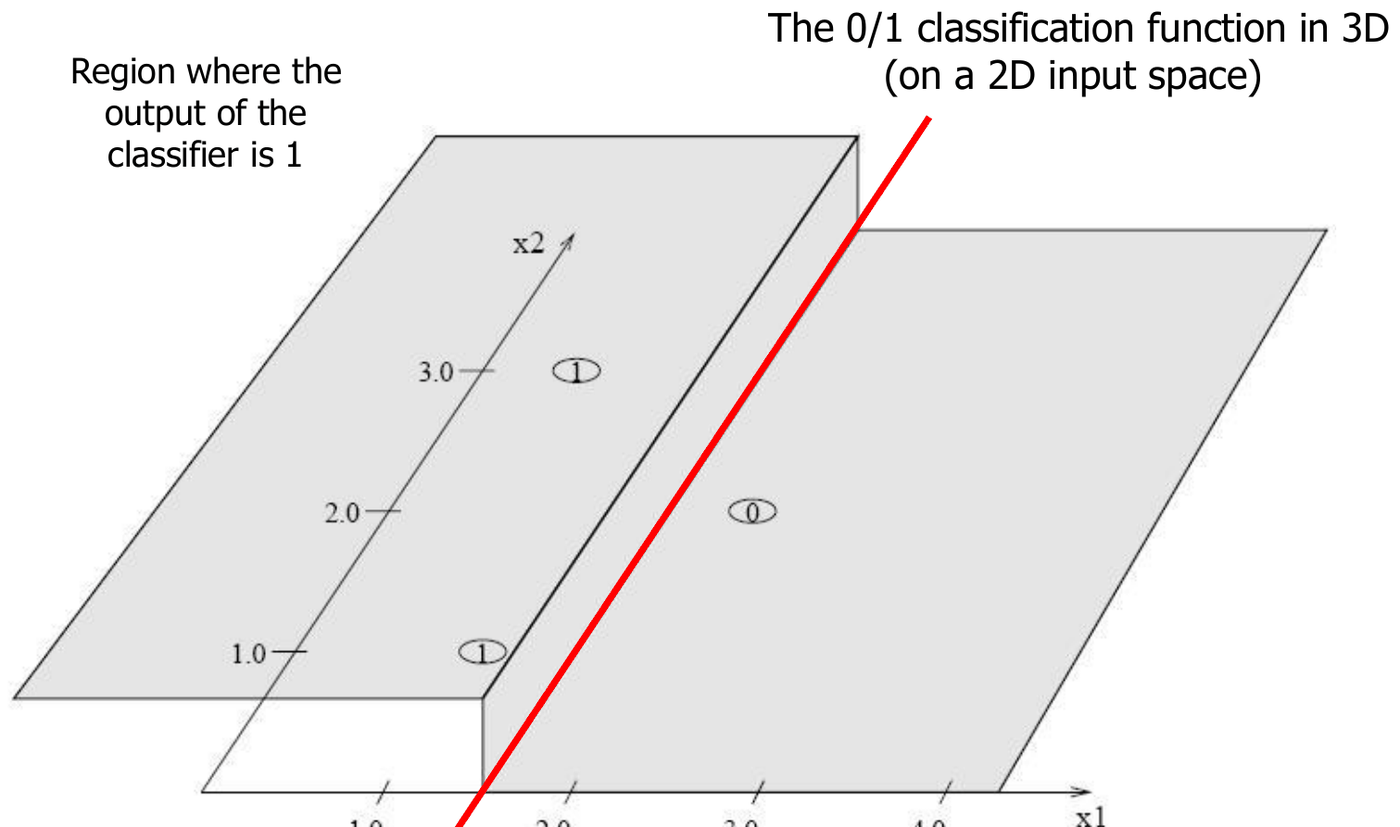
\includegraphics[width=0.77\linewidth,height=0.42\textheight,keepaspectratio]{images/03-l23_classificatore-3d.png}
\caption{La stessa funzione di classificazione vista in 3D: è una funzione ``a
gradino'' che vale 1 in una regione e 0 nell'altra.}
\end{figure}

\subsubsection{Regressione}\label{regressione}

La \textbf{regressione} è la stima di una funzione a valori reali sulla
base di un insieme finito di \textbf{campioni rumorosi}: si conoscono
coppie \((\mathbf{x}, f(\mathbf{x}) + \text{rumore})\). È una forma di
\emph{curve fitting} (in una dimensione nell'esempio, a \(k\) dimensioni
in generale).

\begin{boxexample}{Esercizio di regressione}

Dati i punti \((1;\,2{,}1)\), \((2;\,3{,}9)\), \((3;\,6{,}1)\),
\((4;\,8{,}4)\), \((5;\,9{,}8)\), qual è \(f\)? Viene spontaneo
ipotizzare \(f(x) = 2x\), che ha errori piccoli su tutti i punti. Ma
come abbiamo fatto a sceglierla? E come lo farebbe una macchina (ad
esempio una rete neurale)? È esattamente ciò che l'algoritmo di
apprendimento deve formalizzare.

\end{boxexample}

\begin{figure}[htbp]
\centering
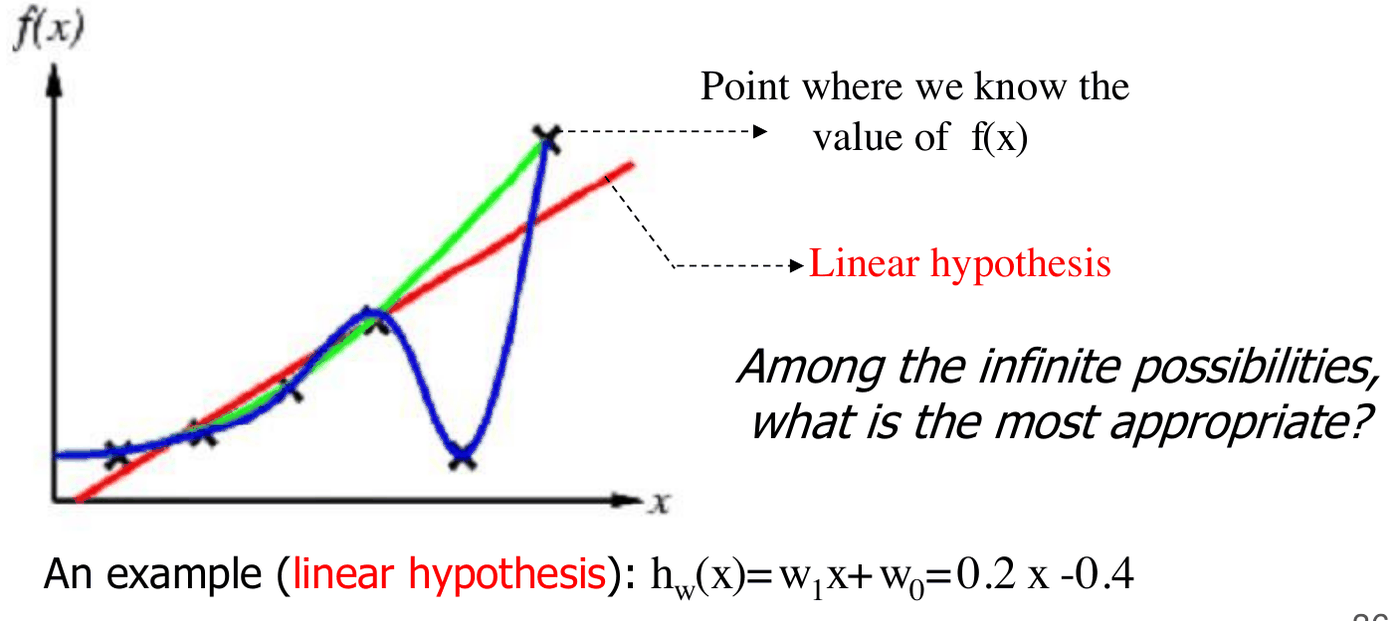
\includegraphics[width=0.77\linewidth,height=0.42\textheight,keepaspectratio]{images/03-l23_regressione.png}
\caption{Tra le infinite funzioni compatibili con i dati, qual è la più
appropriata?}
\end{figure}

La figura pone la domanda chiave: tra le infinite possibilità, quale
funzione scegliere? La curva blu passa esattamente per tutti i punti ma
oscilla in modo innaturale; la retta rossa
(\(h_\mathbf{w}(x) = w_1 x + w_0 = 0{,}2x - 0{,}4\)) commette piccoli
errori ma è molto più semplice. Questo dilemma è il cuore del problema
della \textbf{generalizzazione}.

\subsubsection{Altri paradigmi}\label{altri-paradigmi}

\begin{itemize}
\tightlist
\item
  \textbf{Semi-supervised learning}: combina esempi etichettati e non
  etichettati.
\item
  \textbf{Self-supervised learning}: è un apprendimento supervisionato
  in cui le etichette vengono \textbf{generate automaticamente dalla
  struttura stessa dei dati}, senza etichettatura manuale. Il modello
  viene \textbf{pre-addestrato} su grandi quantità di dati non
  etichettati, imparando rappresentazioni generali, che poi si adattano
  a task specifici con il \textbf{fine-tuning}. Esempi attuali, alla
  base degli LLM:

  \begin{itemize}
  \tightlist
  \item
    la \textbf{predizione della parola successiva} in un testo, cioè
    l'apprendimento self-supervised \textbf{autoregressivo} della
    famiglia GPT (\emph{Generative Pre-trained Transformer}, OpenAI);
  \item
    la ricostruzione di \textbf{parole mascherate} (BERT, Google);
  \item
    per le immagini, i \textbf{masked autoencoder} (Meta), che
    ricostruiscono porzioni nascoste dell'immagine.
  \end{itemize}
\item
  \textbf{Reinforcement learning}: apprendimento con un ``critico'' che
  dice giusto/sbagliato. L'algoritmo apprende una \textbf{politica} su
  come agire date le osservazioni del mondo; ogni azione ha un impatto
  sull'ambiente, che fornisce un feedback. Non ci sono esempi
  passo-passo; l'obiettivo è il \emph{decision-making}, ed è molto usato
  nella AI moderna.
\end{itemize}

\subsection{Modello}\label{modello}

Il \textbf{modello} cattura le relazioni tra i dati (in base al task)
attraverso un ``linguaggio'' (numerico, simbolico, \ldots), legato alla
rappresentazione usata. Soprattutto, \textbf{il modello definisce la
classe di funzioni che la macchina può implementare}: lo \textbf{spazio
delle ipotesi}. Ad esempio, l'insieme delle funzioni
\(h(\mathbf{x}, \mathbf{w})\) al variare del parametro \(\mathbf{w}\).

\begin{boxdefinition}{Terminologia di base}

\begin{itemize}
\tightlist
\item
  \textbf{Esempio di training} (supervisionato): coppia
  \((\mathbf{x}, f(\mathbf{x}) + \text{rumore})\), dove \(\mathbf{x}\) è
  il vettore delle feature e \(d = f(\mathbf{x}) + \text{rumore}\) è il
  \textbf{target}.
\item
  \textbf{Funzione target} \(f\): la vera funzione (sconosciuta).
\item
  \textbf{Ipotesi} \(h\): una funzione proposta, che si ritiene simile a
  \(f\); un'espressione in un dato linguaggio che descrive le relazioni
  tra i dati.
\item
  \textbf{Spazio delle ipotesi} \(H\): l'insieme di tutte le ipotesi che
  l'algoritmo di apprendimento può, in linea di principio, produrre.
\end{itemize}

\end{boxdefinition}

Alcuni esempi di rappresentazioni diverse:

\begin{itemize}
\tightlist
\item
  \textbf{Modelli lineari}: \(H\) è uno spazio parametrizzato in modo
  \textbf{continuo}, e ogni assegnamento di \(\mathbf{w}\) è un'ipotesi
  diversa. Esempi: il classificatore binario
  \(h(\mathbf{x}) = \operatorname{sign}(\mathbf{w}^T\mathbf{x} + w_0)\)
  o la regressione lineare semplice \(h_\mathbf{w}(x) = w_1 x + w_0\)
  (es. \(2x + 150\)).
\item
  \textbf{Regole simboliche}: \(H\) è \textbf{discreto}, ad esempio ``se
  \(x_1 = 0\) e \(x_2 = 1\) allora \(h(\mathbf{x}) = 1\), altrimenti
  \(0\)''.
\item
  \textbf{Modelli probabilistici}: stimano \(p(\mathbf{x}, y)\).
\item
  \textbf{K-nearest neighbors} (regressione): predice la media dei
  valori \(y\) dei vicini più prossimi (modello basato sulla memoria).
\item
  \textbf{Reti neurali}: al di là dell'ispirazione biologica, sono un
  modello computazionale capace di approssimare relazioni complesse e
  \textbf{non lineari} tra input e output. Anche esse, ancora una volta,
  definiscono una \textbf{classe di funzioni}.
\end{itemize}

I principali paradigmi (linguaggi per \(H\)) sono:

{\def\LTcaptype{none} % do not increment counter
\begin{longtable}[]{@{}
  >{\raggedright\arraybackslash}p{(\linewidth - 2\tabcolsep) * \real{0.5000}}
  >{\raggedright\arraybackslash}p{(\linewidth - 2\tabcolsep) * \real{0.5000}}@{}}
\toprule\noalign{}
\begin{minipage}[b]{\linewidth}\raggedright
Paradigma
\end{minipage} & \begin{minipage}[b]{\linewidth}\raggedright
Esempi
\end{minipage} \\
\midrule\noalign{}
\endhead
\bottomrule\noalign{}
\endlastfoot
\textbf{Simbolici / a regole} (\(H\) discreto) & congiunzioni di
letterali, alberi di decisione, grammatiche induttive, algoritmi
evolutivi, Inductive Logic Programming \\
\textbf{Sub-simbolici} (\(H\) continuo) & analisi discriminante lineare,
regressione lineare multipla, LTU, reti neurali, metodi kernel (SVM) \\
\textbf{Probabilistici / generativi} & modelli parametrici tradizionali,
reti bayesiane, Naïve Bayes, modelli di Markov, HMM \\
\textbf{Instance-based} & nearest neighbor \\
\end{longtable}
}

Alcuni modelli possono essere espressi in più linguaggi diversi.

\begin{boxtheorem}{No Free Lunch Theorem}

Non esiste un metodo di apprendimento universalmente ``migliore'' (senza
alcuna conoscenza, per tutti i problemi): se un algoritmo ottiene
risultati superiori su alcuni problemi, deve pagarlo con risultati
inferiori su altri (Devroye 1982; Wolpert e Macready 1997).

\end{boxtheorem}

Per questo il corso fornisce sia un \textbf{insieme di modelli} sia gli
\textbf{strumenti critici per confrontarli}. Tuttavia i modelli
\emph{non} sono tutti equivalenti: differiscono molto per
\textbf{flessibilità} (capacità, in linea di principio, di approssimare
funzioni arbitrarie, non solo lineari) e per il \textbf{controllo della
complessità}. Modelli flessibili e principi per controllarne la
complessità sono il nucleo del ML.

\subsection{Algoritmo di
apprendimento}\label{algoritmo-di-apprendimento}

L'algoritmo di apprendimento, sulla base di dati, task e modello, esegue
una \textbf{ricerca (euristica) nello spazio delle ipotesi \(H\)} per
trovare l'ipotesi migliore, cioè la migliore approssimazione della
funzione target sconosciuta. Tipicamente cerca la \(h\) con
\textbf{errore minimo}: i parametri liberi del modello vengono adattati
al task (il miglior \(\mathbf{w}\) nei modelli lineari, le migliori
regole nei modelli simbolici\ldots). Nell'esempio di regressione, la
scelta \(w_1 = 2\), \(w_0 = 0\) è il risultato di questa ricerca.

\begin{figure}[htbp]
\centering
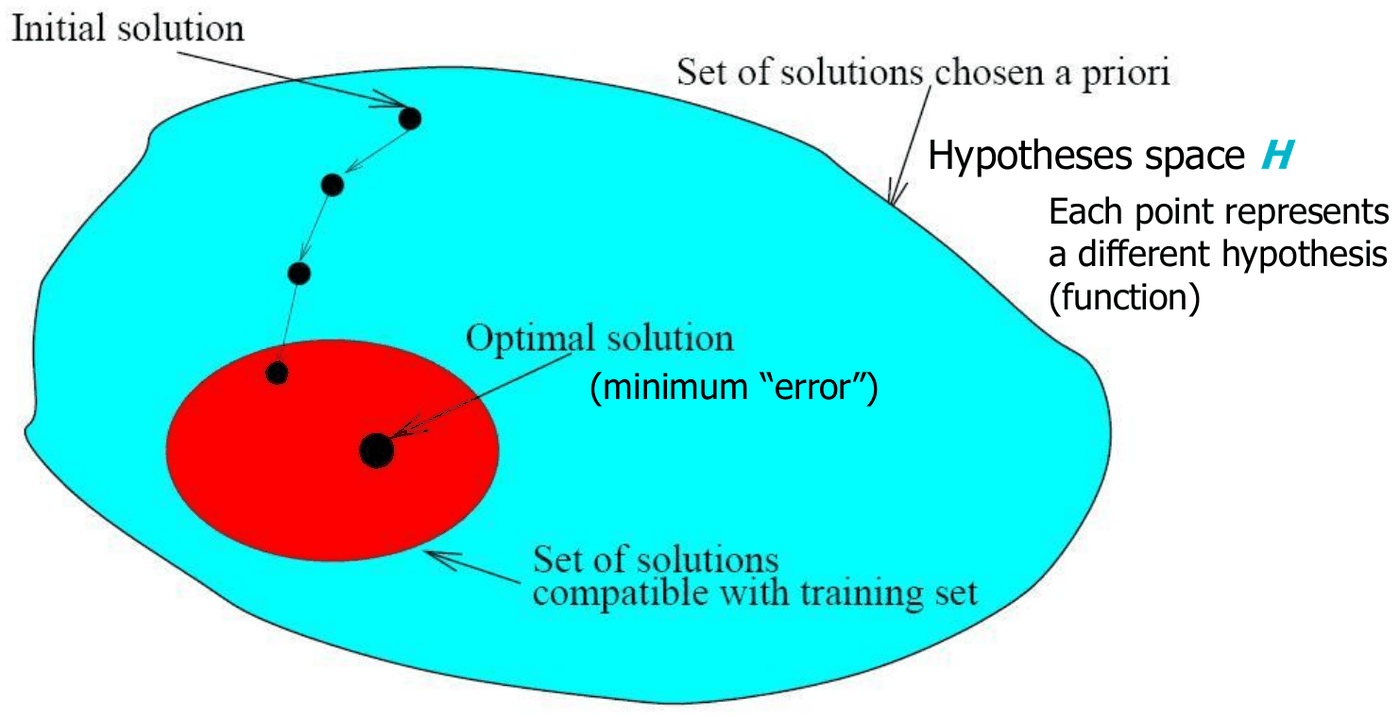
\includegraphics[width=0.77\linewidth,height=0.42\textheight,keepaspectratio]{images/03-l23_ricerca-ipotesi.png}
\caption{L'apprendimento come ricerca nello spazio delle ipotesi: ogni punto è
una funzione diversa; si parte da una soluzione iniziale e si procede,
tipicamente con ricerca locale, verso quella a errore minimo.}
\end{figure}

\(H\) può non coincidere con l'insieme di tutte le funzioni possibili e
la ricerca non può essere esaustiva: servono delle \textbf{assunzioni},
e qui entra in gioco il \textbf{bias induttivo}.

A seconda del contesto, ``apprendimento'' prende nomi diversi:
\textbf{inferenza} (statistica), \textbf{abduzione/induzione} (logica),
\textbf{adattamento} (biologia, sistemi), \textbf{ottimizzazione}
(matematica), \textbf{addestramento/training} (reti neurali),
\textbf{approssimazione di funzioni} (matematica), regressione,
\emph{curve fitting}.

Dopo questi quattro ingredienti restano tre concetti da discutere: il
\textbf{bias induttivo}, la \textbf{loss} e la
\textbf{generalizzazione}.

\section{Il bias induttivo}\label{il-bias-induttivo}

Per costruire un modello e un algoritmo di apprendimento dobbiamo fare
\textbf{assunzioni} sulla natura della funzione target. Queste possono
riguardare:

\begin{itemize}
\tightlist
\item
  \textbf{vincoli sul modello}, cioè sullo spazio delle ipotesi \(H\)
  (l'insieme delle ipotesi che possiamo esprimere): è il
  \textbf{language bias};
\item
  \textbf{vincoli o preferenze nell'algoritmo di apprendimento}, cioè
  nella strategia di ricerca: è il \textbf{search bias};
\item
  entrambi.
\end{itemize}

Vedremo che queste assunzioni sono \textbf{indispensabili} per ottenere
un modello utile, cioè capace di generalizzare. Lo studiamo con esempi
in spazi di ipotesi discreti, imparando un \textbf{concetto} (una
funzione booleana), come in Mitchell cap. 2 (es.
\(h_{cat}(\mathbf{x}) = 1\) se l'animale \(\mathbf{x}\) è un gatto,
\(0\) altrimenti).

\subsection{Imparare funzioni booleane: un problema mal
posto}\label{imparare-funzioni-booleane-un-problema-mal-posto}

Supponiamo di voler imparare una funzione booleana sconosciuta
\(y = f(x_1, x_2, x_3, x_4)\) da 7 esempi.

\begin{figure}[htbp]
\centering
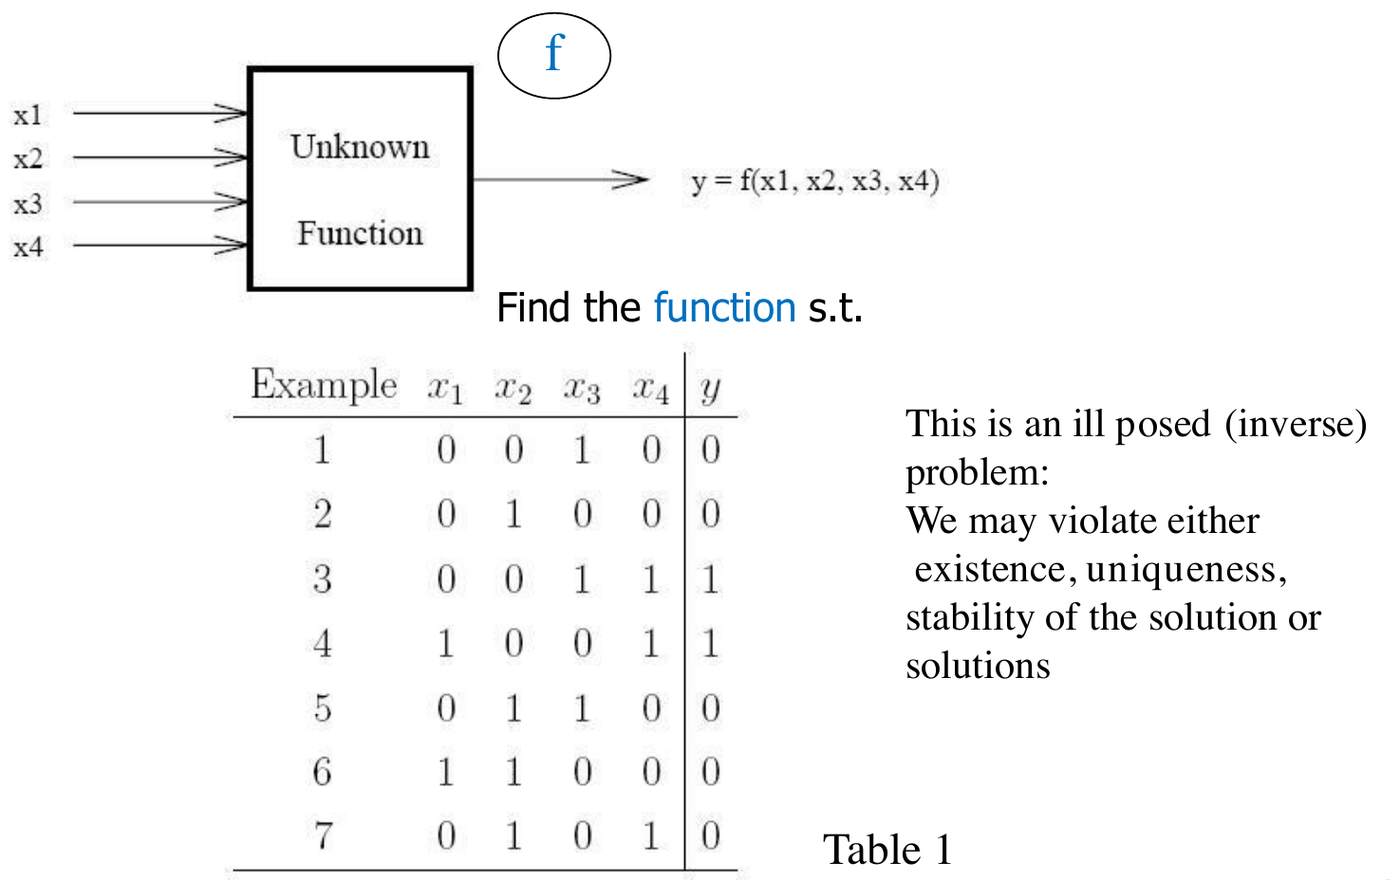
\includegraphics[width=0.77\linewidth,height=0.42\textheight,keepaspectratio]{images/03-l23_funzioni-booleane.png}
\caption{Apprendere una funzione booleana di quattro variabili da sette esempi.}
\end{figure}

Si tratta di un \textbf{problema (inverso) mal posto}: la soluzione può
violare esistenza, unicità o stabilità. Con 4 input binari esistono
\(2^4 = 16\) possibili istanze di input e quindi \(2^{16} = 65536\)
possibili funzioni booleane. Non possiamo sapere quale sia quella
corretta finché non vediamo \textbf{tutte} le coppie input-output: dopo
7 esempi restano ancora \(2^9 = 512\) possibilità (le 9 istanze non
viste possono avere output qualsiasi).

In generale, per input e output binari con dimensione dell'input \(n\):
\[
|H| = 2^{\#\text{istanze di input}} = 2^{2^n}.
\]

Un modello che usa tutto questo spazio è una \textbf{lookup table}: un
\emph{rote learner} che memorizza gli esempi e classifica \(\mathbf{x}\)
solo se coincide con un esempio già visto (altrimenti ``nessuna
risposta''). \textbf{Nessun bias induttivo → nessuna generalizzazione.}

\subsection{Restringere lo spazio: le regole
congiuntive}\label{restringere-lo-spazio-le-regole-congiuntive}

Introduciamo un \textbf{language bias}: consideriamo solo \textbf{regole
congiuntive}, cioè congiunzioni (AND) di letterali, come \(h_1 = l_2\),
\(h_2 = l_1 \wedge l_2\), \(h_3 = \text{true}\),
\(h_4 = \neg l_1 \wedge l_2\). Ad esempio ``se \(x_2 = 1\) allora
\(h(\mathbf{x}) = 1\), altrimenti \(0\)''.

Il numero di ipotesi semanticamente distinte crolla: per ognuna delle
\(n\) posizioni possiamo avere \(l_i\), \(\neg l_i\) oppure ``non
importa'', da cui \(3^n\) ipotesi, più 1 perché tutte le congiunzioni
che contengono \(l_i \wedge \neg l_i\) equivalgono a ``false''. Con
\(n = 4\) si passa da 65536 a \(3^4 + 1 = 82\) ipotesi.

\begin{boxdefinition}{Consistenza e Version Space}

Un'ipotesi \(h\) è \textbf{consistente} con il training set TR se
\(h(\mathbf{x}) = d(\mathbf{x})\) per ogni esempio
\(\langle \mathbf{x}, d(\mathbf{x})\rangle \in TR\).

Il \textbf{version space} \(VS_{H,TR}\) è il sottoinsieme delle ipotesi
di \(H\) consistenti con tutti gli esempi di training.

\end{boxdefinition}

In questo spazio ridotto esistono algoritmi efficienti (Mitchell cap. 2)
che trovano il version space senza enumerare tutte le ipotesi.

\subsection{L'unbiased learner}\label{lunbiased-learner}

L'assunzione congiuntiva è però troppo restrittiva: se il concetto
target non è in \(H\) non può essere rappresentato. Ad esempio ``se
\(x_1 = 1\) \textbf{oppure} \(x_2 = 1\) allora 1'' non è una
congiunzione.

L'idea opposta è scegliere un \(H\) capace di esprimere \textbf{ogni
concetto insegnabile}: l'insieme di tutti i sottoinsiemi dello spazio
degli input \(X\), cioè l'insieme delle parti \(\mathcal{P}(X)\)
(disgiunzioni, congiunzioni, negazioni). Con \(n = 10\) input binari,
\(|X| = 2^{10} = 1024\) e
\(|\mathcal{P}(X)| = 2^{1024} \approx 10^{308}\) concetti --- più degli
atomi dell'universo. \(H\) contiene sicuramente il concetto target. Ma
cosa succede alla generalizzazione?

\begin{boxtheorem}{Un learner senza bias non può generalizzare}

Con un \emph{unbiased learner}, le uniche istanze classificate in modo
non ambiguo dal version space sono gli esempi di training stessi: si
ottiene di nuovo una \textbf{lookup table}.

\textbf{Dimostrazione.} Sia \(x_i\) un'istanza non vista (di test) e sia
\(h \in VS\). Consideriamo \(h'\) identica a \(h\) ovunque tranne che in
\(x_i\), dove \(h'(x_i) \ne h(x_i)\). Poiché \(H\) contiene \emph{tutte}
le funzioni, \(h' \in H\); e poiché \(h\) e \(h'\) coincidono sul
training set, anche \(h' \in VS\). Quindi per ogni ipotesi del VS che
classifica \(x_i\) come positivo ce n'è un'altra che lo classifica
negativo: ogni istanza non vista è classificata 1 da esattamente metà
delle ipotesi del VS e 0 dall'altra metà. Il VS non può dare alcuna
risposta.

\end{boxtheorem}

\begin{boxexample}{Esempio banale}

Un solo input binario \(x\), \(H = \{x, \neg x, 0, 1\}\) (tutte le
funzioni possibili). Il TR contiene solo \(x = 0 \mapsto d = 0\). Il
version space è \(\{x, 0\}\): entrambe valgono 0 in \(x = 0\). Per il
test \(x = 1\), però, \(x\) risponde 1 e \(0\) risponde 0. Non c'è modo
di decidere, a meno di usare tutto \(X\) come training set.

\end{boxexample}

\begin{boxtip}{Futilità dell'apprendimento senza bias}

Un learner che non fa \textbf{alcuna assunzione a priori} sull'identità
del concetto target \textbf{non ha alcuna base razionale} per
classificare istanze non viste. Il bias (di restrizione o di preferenza)
non serve solo per l'efficienza: è \textbf{necessario per la
generalizzazione}. Per imparare senza bias bisognerebbe mostrare ogni
singola istanza di \(X\) come esempio. Il bias però non ci dice ancora
\emph{quale} soluzione generalizza meglio.

\end{boxtip}

\subsection{Sistemi induttivi e deduttivi
equivalenti}\label{sistemi-induttivi-e-deduttivi-equivalenti}

Un modo elegante di vedere il ruolo del bias: un sistema induttivo
(algoritmo di apprendimento che, usando lo spazio delle ipotesi \(H\),
riceve esempi e una nuova istanza e produce una classificazione o ``non
so'') è \textbf{equivalente a un sistema deduttivo} --- un dimostratore
di teoremi --- che riceve gli stessi esempi e la stessa istanza
\textbf{più il bias induttivo come assioma aggiuntivo}. Il bias
induttivo è quindi esattamente l'insieme di assunzioni che rende
``logicamente deducibile'' la classificazione prodotta dal learner.

\begin{figure}[htbp]
\centering
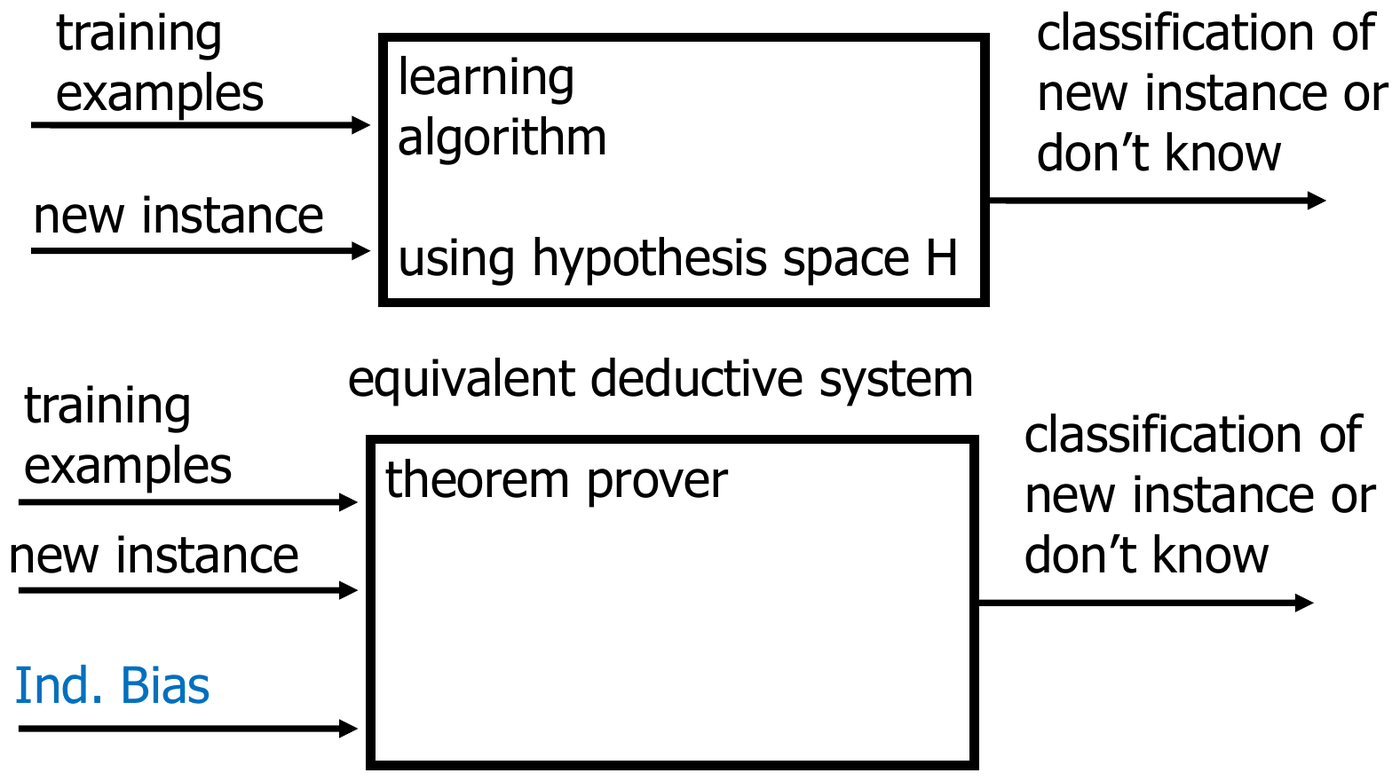
\includegraphics[width=0.80\linewidth,height=0.42\textheight,keepaspectratio]{images/03-l23_sistemi-induttivi.png}
\caption{Il bias induttivo rende un sistema induttivo equivalente a un sistema
deduttivo.}
\end{figure}

\subsection{Language bias o search
bias?}\label{language-bias-o-search-bias}

Nel ML moderno si preferisce in genere il \textbf{search bias}. Si usano
approcci flessibili, con spazi di ipotesi molto espressivi e capacità di
approssimazione universale (reti neurali, alberi di decisione), evitando
il language bias e quindi \textbf{senza escludere a priori} la funzione
target. Il bias induttivo resta, ma è affidato alla \textbf{strategia di
ricerca} dell'algoritmo di apprendimento, in pratica usando una ricerca
\textbf{incompleta} (che privilegia certe soluzioni rispetto ad altre).

\begin{boxabstract}{Conclusioni sul bias induttivo}

\begin{itemize}
\tightlist
\item
  Apprendere senza bias non permette di estrarre regolarità dai dati: si
  ottiene una lookup table, senza generalizzazione.
\item
  \textbf{Ogni approccio di ML allo stato dell'arte ha un bias
  induttivo.}
\item
  Il problema è caratterizzare il bias dei diversi modelli e algoritmi.
\end{itemize}

\end{boxabstract}

\begin{figure}[htbp]
\centering
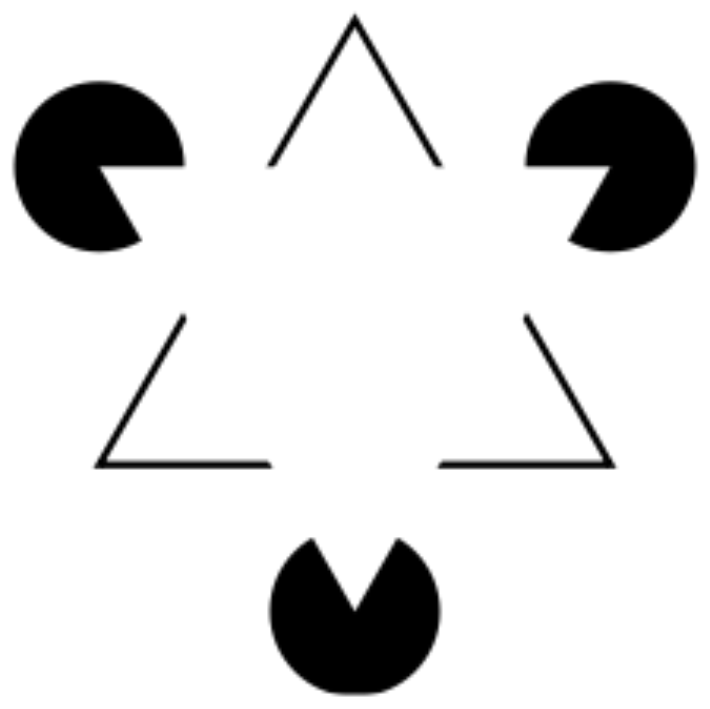
\includegraphics[width=0.37\linewidth,height=0.42\textheight,keepaspectratio]{images/03-l23_kanizsa.png}
\caption{Il triangolo di Kanizsa: un esempio di bias percettivo del nostro
sistema visivo, che ``completa'' forme non presenti.}
\end{figure}

\section{Task e funzioni di loss}\label{task-e-funzioni-di-loss}

Abbiamo detto di voler trovare una ``buona'' approssimazione di \(f\).
Ma come si misura la qualità dell'approssimazione? Il modello produce
\(h(\mathbf{x})\) per l'input \(\mathbf{x}\), e vogliamo misurare la
``distanza'' tra \(h(\mathbf{x})\) e il target \(d\). Si usa una
\textbf{funzione di loss} (``interna'')
\(L(h_\mathbf{w}(\mathbf{x}), d)\) calcolata sul singolo pattern: un
valore alto indica un'approssimazione scarsa.

\begin{boxdefinition}{Errore (Rischio, Loss)}

L'\textbf{errore} è un valore atteso della loss \(L\), ad esempio la sua
media sugli \(l\) campioni: \[
\text{Loss}(h_\mathbf{w}) = E(\mathbf{w}) = \frac{1}{l} \sum_{p=1}^{l} L\big(h_\mathbf{w}(\mathbf{x}_p), d_p\big).
\] Serve come \textbf{funzione obiettivo} da minimizzare durante il
training e come misura di controllo dell'errore in fase di test. Per ora
Errore, Rischio e Loss sono considerati sinonimi; le differenze verranno
precisate più avanti.

\end{boxdefinition}

La funzione \(L\) cambia a seconda del task. Vediamo i casi principali
(utili come riferimento futuro).

\subsection{Regressione: errore
quadratico}\label{regressione-errore-quadratico}

\begin{itemize}
\tightlist
\item
  \textbf{Output}: \(d_p = f(\mathbf{x}_p) + e\) (funzione reale più
  errore casuale).
\item
  \textbf{\(H\)}: un insieme di funzioni a valori reali.
\item
  \textbf{Loss}: l'\textbf{errore quadratico}
  \(L(h_\mathbf{w}(\mathbf{x}_p), d_p) = \big(d_p - h_\mathbf{w}(\mathbf{x}_p)\big)^2\).
\item
  La media sul dataset è il \textbf{Mean Squared Error} (MSE).
\end{itemize}

\begin{figure}[htbp]
\centering
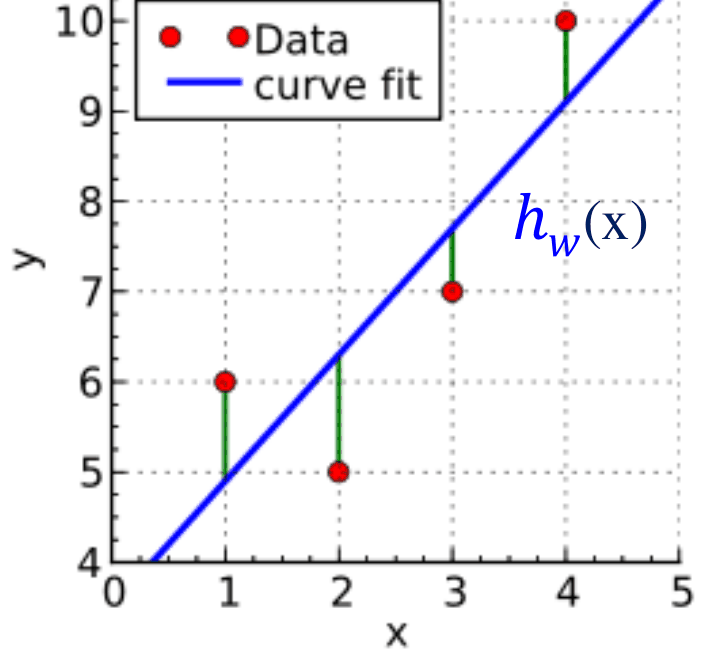
\includegraphics[width=0.43\linewidth,height=0.42\textheight,keepaspectratio]{images/03-l23_mse.png}
\caption{L'MSE è la media dei quadrati dei segmenti verdi, cioè delle distanze
verticali tra i dati (in rosso) e la retta \(h_w(x) = w_1x + w_0\) (in
blu).}
\end{figure}

\[
E(\mathbf{w}) = \frac{1}{l} \sum_{p=1}^{l} \big(y_p - h_\mathbf{w}(\mathbf{x}_p)\big)^2
\] dove \(\mathbf{w}\) sono i parametri liberi del modello lineare
(nella figura i target sono indicati con \(y\)).

\subsection{Classificazione: loss 0/1}\label{classificazione-loss-01}

\begin{itemize}
\tightlist
\item
  \textbf{Output}: ad esempio \(\{0, 1\}\).
\item
  \textbf{\(H\)}: un insieme di funzioni indicatrici.
\item
  \textbf{Loss 0/1}: \[
  L(h_\mathbf{w}(\mathbf{x}_p), d_p) = \begin{cases} 0 & \text{se } h_\mathbf{w}(\mathbf{x}_p) = d_p \\ 1 & \text{altrimenti} \end{cases}
  \]
\item
  La media sul dataset è la \textbf{percentuale di pattern classificati
  male}: se 20 pattern su 100 sono sbagliati si ha il 20\% di errore,
  cioè l'80\% di \textbf{accuratezza}.
\end{itemize}

\subsection{Clustering e vector quantization
(anticipazione)}\label{clustering-e-vector-quantization-anticipazione}

\begin{itemize}
\tightlist
\item
  \textbf{Obiettivo}: partizionare in modo ottimo una distribuzione
  sconosciuta nello spazio degli input in regioni (cluster), ognuna
  approssimata da un \textbf{centro} o \textbf{prototipo}.
\item
  \textbf{\(H\)}: un insieme di \emph{vector quantizer}
  \(\mathbf{x} \mapsto c(\mathbf{x})\), che mappano lo spazio continuo
  in uno discreto.
\item
  \textbf{Loss}: la \textbf{distorsione quadratica}, che misura la
  vicinanza del pattern al centroide del suo cluster: \[
  L(h(\mathbf{x}_p)) = \big(\mathbf{x}_p - h(\mathbf{x}_p)\big) \cdot \big(\mathbf{x}_p - h(\mathbf{x}_p)\big) = \|\mathbf{x}_p - h(\mathbf{x}_p)\|^2.
  \]
\end{itemize}

\subsection{Stima di densità
(anticipazione)}\label{stima-di-densituxe0-anticipazione}

\begin{itemize}
\tightlist
\item
  \textbf{Obiettivo}: stimare una densità da una classe assunta (metodi
  generativi, parametrici).
\item
  \textbf{Output}: una densità, ad esempio una normale
  \(p(\mathbf{x} \mid \mu, \sigma^2)\).
\item
  \textbf{\(H\)}: un insieme di densità (qui \(\mu\) e \(\sigma^2\) sono
  i due parametri sconosciuti).
\item
  \textbf{Loss}: \(L(h(\mathbf{x}_p)) = -\ln h(\mathbf{x}_p)\), legata
  alla \textbf{massimizzazione della (log-)verosimiglianza}: minimizzare
  la somma dei \(-\ln\) equivale a massimizzare il prodotto delle
  probabilità dei dati osservati.
\end{itemize}

\section{Generalizzazione e
validazione}\label{generalizzazione-e-validazione}

Questo è il \textbf{concetto fondamentale del corso}.

\begin{itemize}
\tightlist
\item
  L'\textbf{apprendimento} è la ricerca di una buona funzione in uno
  spazio di funzioni a partire da dati noti, tipicamente minimizzando un
  errore/loss.
\item
  ``Buona'' rispetto all'\textbf{errore di generalizzazione}: quanto
  accuratamente il modello predice su \textbf{dati nuovi} (loss misurata
  su dati nuovi).
\end{itemize}

\begin{boxwarning}{La generalizzazione è il punto cruciale}

È facile \emph{usare} strumenti di ML; è molto più difficile usarli
\emph{bene}. La differenza sta tutta nella generalizzazione.

\end{boxwarning}

Si distinguono due fasi:

\begin{enumerate}
\def\labelenumi{\arabic{enumi}.}
\tightlist
\item
  \textbf{Fase di apprendimento} (\emph{training}, \emph{fitting}): si
  costruisce il modello dai dati noti (i dati di training, più il bias).
\item
  \textbf{Fase predittiva o di test} (\emph{deployment}, uso del modello
  in inferenza): si applica il modello a nuovi esempi. Si prendono nuovi
  input \(\mathbf{x}'\), si calcola la risposta del modello e la si
  confronta con il target \(d'\) che il modello \textbf{non ha mai
  visto}: così si valuta la capacità di generalizzazione.
\end{enumerate}

\begin{boxnote}{Performance nel ML}

Nel ML, ``prestazione'' significa \textbf{accuratezza di
generalizzazione} (o accuratezza predittiva), stimata dall'errore
calcolato su un \textbf{test set} tenuto da parte (\emph{hold out}).

\end{boxnote}

La \textbf{Statistical Learning Theory} (Vapnik) studia le condizioni
matematiche sotto cui un modello è in grado di generalizzare; se ne
vedranno le basi nella prossima lezione.

La valutazione delle prestazioni di un sistema di ML coincide con la
valutazione della sua accuratezza predittiva: in una parola,
\textbf{validazione! validazione! validazione!} Le tecniche di
validazione servono sia a \textbf{valutare} la generalizzazione
(\emph{model assessment}) sia a \textbf{gestirla} (\emph{model
selection}), e saranno l'oggetto della prossima lezione.

\begin{boxnote}{Il costo dell'inferenza}

Anche la sola fase di inferenza (il \emph{mapping} input → output) può
essere costosa quando le richieste sono milioni, come nei servizi di
Google: per questo sono stati progettati chip dedicati come le
\textbf{Tensor Processing Unit} (TPU), pensate originariamente per
TensorFlow.

\end{boxnote}

\begin{boxabstract}{Sintesi}

Il ML costruisce un'ipotesi \(h\) che approssima una funzione
sconosciuta \(f\) a partire da esempi. I suoi ingredienti sono
\textbf{dati} (rappresentazione, codifica, rumore), \textbf{task}
(supervisionato: classificazione e regressione; non supervisionato:
clustering, densità), \textbf{modello} (che definisce lo spazio delle
ipotesi \(H\)), \textbf{algoritmo di apprendimento} (ricerca in \(H\)
dell'ipotesi a errore minimo) e \textbf{validazione}. Senza \textbf{bias
induttivo} non c'è generalizzazione; nel ML moderno si preferisce il
\emph{search bias} con modelli molto espressivi. La qualità si misura
con una \textbf{loss} che dipende dal task (quadratica, 0/1,
distorsione, \(-\ln\)), ma ciò che conta davvero è l'errore sui
\textbf{dati nuovi}.

\end{boxabstract}

\begin{boxquestion}{Possibili domande d'esame}

\begin{itemize}
\tightlist
\item
  Che cos'è il bias induttivo? Qual è la differenza tra language bias e
  search bias?
\item
  Dimostrare che un \emph{unbiased learner} non può generalizzare.
\item
  Quante sono le ipotesi con \(n\) input binari senza vincoli? E con
  sole regole congiuntive?
\item
  Che cos'è il version space?
\item
  Quali loss si usano per regressione, classificazione, clustering e
  stima di densità?
\item
  Cosa si intende per generalizzazione e come si stima?
\end{itemize}

\end{boxquestion}
